\section{\replaced{Layout Fine-Tuning: Workflow and Interface}{Layout Fine-tuning For Node-Link Diagrams}}
\replaced{We have designed and implemented an end-to-end tool for exemplar-based layout fine-tuning to reduce the manual workload of refining layout by suggesting fine-tuning candidates (similar substructures) and transferring user modifications to those candidates (Figure~\ref{fig:workflow}).}
{
An automatically generated node-link diagram may not be satisfying. For instance, a force-directed layout may lead to node overlapping or distorted cycle paths.
Fine-tuning can reduce visual clutter and improve visual aesthetics.
Transferring user modifications to other similar substructures in the entire graph can further gain performance improvement. After the exemplar is specified as the source substructure, 
substructures similar to the exemplar are retrieved in the underlying graph. 
The user modification on the exemplar is transferred onto similar substructures (the target substructures).
}
% JC: moved to Workflow
%After user's specifying an exemplar, 
%our approach retrieves
%substructures similar to the exemplar in the underlying graph. 
%Then our new modification transfer algorithm 
%(described in 
%(See
%Section~\ref{sec:ModificationTransfer}) transfers the user modification on the exemplar to those similar substructures (the target substructures).
%JC: these are not used in this Section? moved to Section 4.
%\added[id=pan]{
%We define 
%some 
%terms in Table~\ref{tab:terms}. 
%JC. moved to table caption.. 
%Here an unlabeled and undirected graph can be denoted as $G=(V, E)$, where $V=\left\{v_1, v_2, \ldots, v_n\right\}, v_i \in \mathbb{R}^2$ are the positions of a set of $n$ nodes and $E=\left\{e_1, e_2, \ldots, e_m\right\}$ is a set of $m$ edges in $G$.
%}


% JC: I like pipeline better. let you decide 
% OR removing this does not cause any thing.
%\subsection{\replaced[id=pan]{\textcolor{myred}{Workflow}}{Pipeline}}
% JC: repetitive and combined with the first sentence in this section.
%Our approach is designed to reduce the manual workload of refining layout by suggesting fine-tuning candidates (similar substructures) and transferring user modifications to the candidates. 

%JC. remove okay? this part is pretty much the same as the four steps below. % 
%\textcolor{myred}{
%To use approach, the user first specifies an exemplar, our tool retrieves substructures similar to the exemplar in the underlying graph. Then our new modification transfer algorithm 
%(See Section~\ref{sec:ModificationTransfer}) transfers the user modification on the exemplar to those similar substructures (the target substructures).
%}
Our workflow has four steps:
%(Figure~\ref{fig:workflow}):
\begin{compactenum}[\textbf{Step} 1.]
    % \item The embeddings of nodes in the entire graph are calculated to retrieve similar structures. \added[id=pan]{\highlight{A node-link diagram is initialized with a pre-computed layout.}} (Figure~\ref{fig:workflow}a).
    \item
    Our algorithm calculates the node embedding of the entire graph to retrieve similar structures (Figure~\ref{fig:workflow}a). \added{A node-link diagram is generated with an initial layout of the entire graph.}
    \item
    The user specifies an exemplar from the entire graph.
    \replaced{
    Our similar structure-query technique using the method in~\cite{DBLP:journals/tvcg/ChenGHPNXZ19} retrieves several target substructures topologically similar to the exemplar (Figure~\ref{fig:workflow}b).}{Similar substructures are retrieved (Figure~\ref{fig:workflow}b).} The user can also specify target substructures from the node-link diagram.
    \item 
    \replaced{
    The user modifies the exemplar's layout. 
    Our modification transfer algorithm transfers the modifications to target substructures (Figure~\ref{fig:workflow}c).
    }{ Markers are generated by automatic graph matching methods or specified by the user on the exemplar and its counterparts, and then modifies the exemplar's layout. The modifications are transferred onto target substructures (Figure~\ref{fig:workflow}c).}
    \item 
    %JC: is this okay?
    %Modified substructures are merged into the entire layout with a global optimization to smooth the borders. 
    Our algorithm merges the modified substructures into the original
    graph through global optimization to smooth the boundaries. 
    The user can iterate from \textit{Step} $2$ to \textit{Step} $4$ to fine-tune the layout (Figure~\ref{fig:workflow}d).
    %Operations are iterated from Step 2 to Step 4 as needed (Figure~\ref{fig:workflow}d). 
\end{compactenum}

\begin{figure}[!tp] % JC moved it to the top
    \centering
    \setlength{\belowcaptionskip}{-5pt}
    \includegraphics[width=1\columnwidth]{picture/newworkflow}
    \caption{
    Workflow of our end-to-end system:
    (a) pre-computing node embeddings and laying-out
    a node-link diagram; (b) detecting similar target substructures with a specified exemplar; (c) transferring user modifications to similar substructures; (d) merging modified substructures into the entire layout with global optimization.}
    \label{fig:workflow}
\end{figure}




\subsection{Step 1. Node-embedding-based Representations}
Our approach uses a node-embedding technique to embed a node into a low-dimensional vector subject to its local topology. For a given exemplar, we employ the node-embedding-based representation to represent and retrieve similar substructures from the entire graph. In this way, we simplify the subgraph-retrieving problem to a similar multidimensional data-searching problem. 
%Note that 
Though various node-embedding representations~\cite{DBLP:conf/kdd/DonnatZHL18, DBLP:conf/kdd/GroverL16, DBLP:conf/cikm/HeimannSSK18, DBLP:journals/cn/MarcusS12, 10.1145/3097983.3098061} 
are compatible with our approach,
%Our implementation 
we leverage GraphWave~\cite{DBLP:conf/kdd/DonnatZHL18} \added[id=pan]{following the study conducted in~\cite{DBLP:journals/tvcg/ChenGHPNXZ19}.} \deleted[id=pan]{Section~\ref{sec:discussion} discusses the performance with different representations.}
\added[id=pan]{We pre-compute node embeddings because 
%JC
%some embedding techniques are 
this process is
time-consuming.}

\subsection{Step 2. Specifying Exemplar and Targets} \label{sec:retrieval}
The user can specify a substructure using the lasso interactions in the node-link diagram
\deleted[id=pan]{
After this,
%the exemplar is specified, 
candidate nodes that have similar embeddings with the exemplar's nodes are identified by the $k$-nearest neighbors algorithm. 
The connected substructures of candidate nodes thus induced are denoted as candidate substructures.
Similar substructures are further filtered by limiting their number of nodes and are ranked by Weisfeiler-Lehman similarity~\cite{DBLP:conf/nips/TogninalliGLRB19}.}
\added{(Figure~\ref{fig:interface}a).
We then use the similar structure-query technique 
in~\cite{DBLP:journals/tvcg/ChenGHPNXZ19} to retrieve a set of substructures that are potentially similar to the exemplar (Figure~\ref{fig:interface}c).}
Four parameters are used in the searching process.
The parameter $k$ is used in the $k$-nearest neighbors algorithm for retrieving similar nodes. 
\added[id=pan]{A large $k$ may introduce many candidate nodes in a huge connected substructure; it will be filtered out by parameter $max$. On the other hand, 
a small $k$ limits the number of candidate nodes, so that the probability of forming a connected substructure is small. The parameter $k$ should be tuned 
%JC. if you say heuristically, you will have to describe the heuristics, which means rules to follow. 
%heuristically.
interactively.
}
We eliminate
similar substructures whose node number is less than the \textit{minimum count} ($min$) or more than the \textit{maximum count} ($max$).
%are eliminated. 
\added[id=pan]{We suggest setting $min$ and $max$ 
to be 
close to the number of nodes in the exemplar (e.g., set $min$ to be half $\# nodes$ and $max$ to be twice $\# nodes$), so as to generate substructures of similar scale to the exemplar.} 
%The algorithm 
We also remove substructures whose Weisfeiler-Lehman similarity is less than the \textit{minimum similar threshold} ($\epsilon$).
% Identified similar substructures are displayed in order of Weisfeiler-Lehman similarity to the exemplar (Figure~\ref{fig:interface}c). 

% \added[id=pan]{
% Because node embeddings often capture nodes' contextual information, the retrieval algorithm actually detects contextually similar structures rather than topologically similar structures. 
% When the exemplar has few edges linked to the rest of the entire graph, thus the embeddings capture mainly the exemplar's information rather than the context, so that the approach can work well.
% } 

Also, we let the user specify additional structures in the node-link diagram using lasso interactions. We regard both retrieved substructures and user-specified substructures as target substructures. 

\begin{figure}[!tp]
    \centering
    \setlength{\belowcaptionskip}{-5pt}
    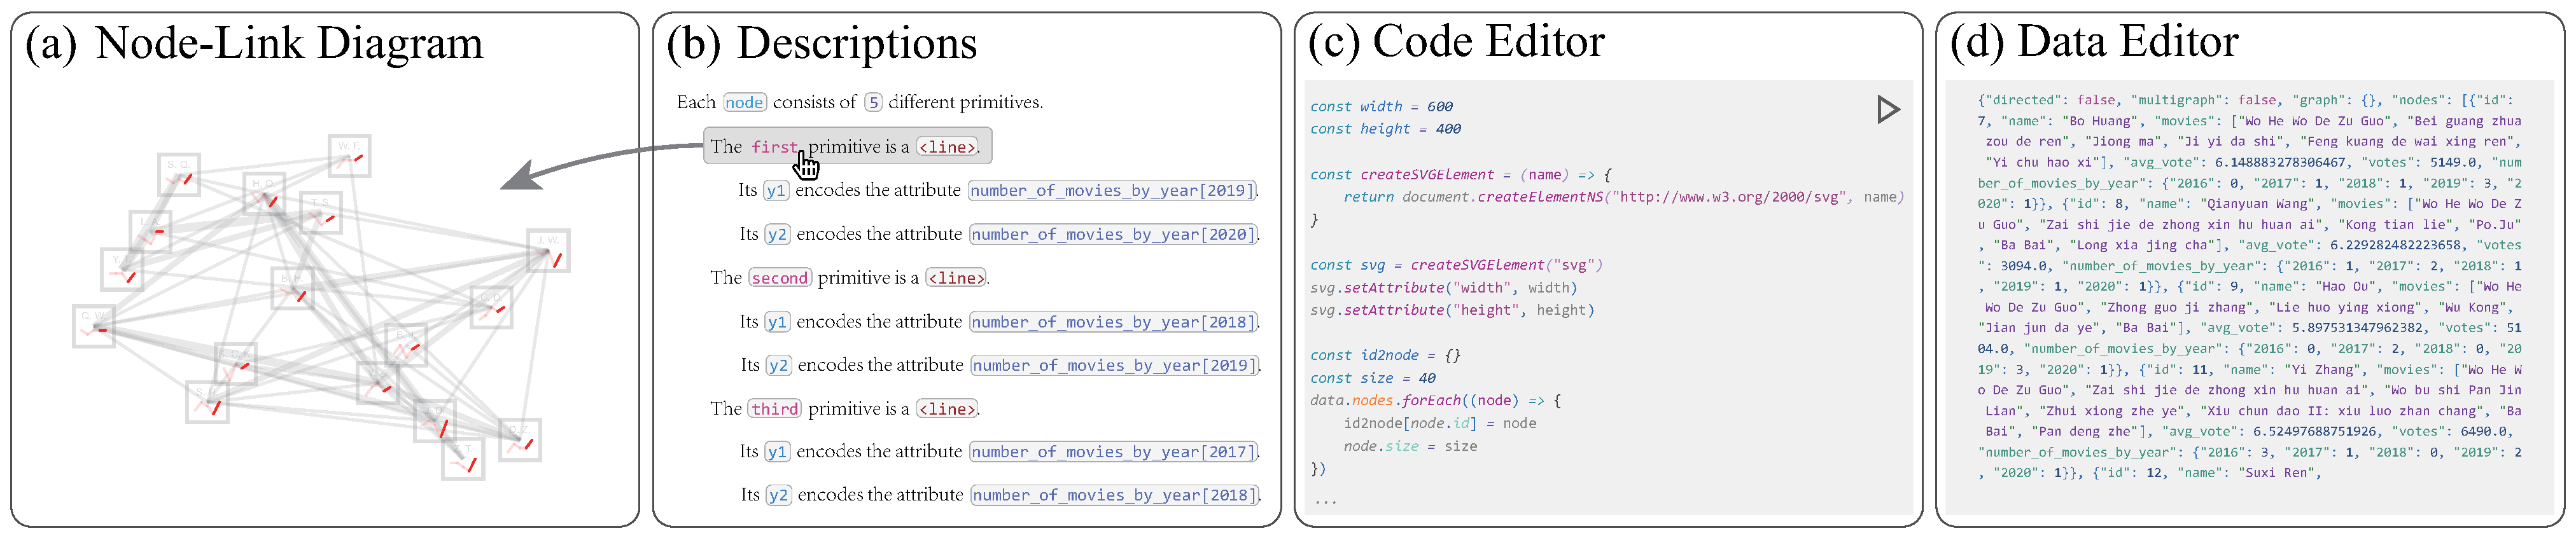
\includegraphics[width=1\columnwidth]{picture/interface}
    \caption{The user interface of our prototype system:
    (a) an exemplar view; (b) a control panel; (c) a suggestions gallery; (d) a node-link view; (e) a modification history view.}
    \label{fig:interface}
\end{figure}

\subsection{Step 3. User-driven Fine-tuning} \label{sec:tuning}
Our approach uses dragging interaction to interactively manipulate the exemplar's layout.
\added{The modification transfer algorithm described in Section~\ref{sec:ModificationTransfer} can transfer the exemplar's layout modifications to target substructures' layouts.
We design an interaction mode called ``format painter" (inspired by operations in Microsoft Word) to perform the modification transfer. 
%It is inspired by the ``format painter" in Microsoft Word.
After modifying the exemplar's layout, the user can transfer modifications to other target substructures using the ``copy'' and ``paste'' buttons. Our approach records modifications after the user clicks the ``copy'' button and transfers modifications into target substructures after the user clicks the ``paste'' button.}
\deleted{Then, we determine a set of markers to initialize the modification transfer. Many graph matching methods are represented for constructing nodes correspondences.
We test 6 graph matching methods to build correspondences: GA (graduated assignment)~\cite{gold1996graduated}, PM (probabilistic matching)~\cite{zass2008probabilistic}, SM (spectral matching)~\cite{leordeanu2005spectral}, SMAC (spectral matching with affine constraints)~\cite{cour2007balanced}, RRWM (re-weighted random walk matching)~\cite{cho2010reweighted} and FGMU (factorized graph matching for undirected graphs)~\cite{zhou2012factorized}. 
Three cases are performed with: three small collaboration networks taken from the Visualization-Publication dataset~\cite{Isenberg:2017:VMC}, three substructures taken from the Finan512 dataset~\cite{DBLP:journals/jgo/SoperWC04} (Figure~\ref{fig:correspondence}), and three circle structures taken from the Power-Network dataset~\cite{nr}. Our approach utilizes their results as markers in the modifications transferring. However, unpleasant results may be generated because these methods build correspondences for all nodes even if the nodes are not well matched. Our approach removes several poorly matched correspondences and selects others as markers by using the technique described in Algorithm~\ref{alg:corrselection}. In practice, FGMU is employed in our approach to generate markers. Note that, our approach also supports specifying markers manually to match user preferences.}

\deleted{The layout of the exemplar and target substructures are generated with the same algorithm before constructing correspondences, leading to more satisfying correspondences. In our implementation, FM$^3$~\cite{hachul2004drawing} is employed.}

\deleted{With specified markers, a ``format painter" interaction mode is designed to fulfill the modification transfer. The ``format painter" interaction is inspired by the ``Format Painter" in Microsoft Word:
after modifying the exemplar's layout, the ``format painter" can transfer modifications to other target substructures. 
New node positions of the target substructure are computed. After that, another substructure can be selected for ``painting".}


\subsection{Step 4. Global Layout Optimization}
The exemplar and target substructures are parts of the entire graph. 
Directly merging 
%JC
%\textcolor{myred}{layout-modified structures} 
the modified layout
into the entire graph may lead to abrupt boundaries of the modified substructures (Figure~\ref{fig:finan512detail}b). Thus, we perform a global optimization to preserve the smooth boundaries of the modified substructures (Figure~\ref{fig:finan512detail}c).
The optimization process is similar to the \textit{deforming} step,
%in Section~\ref{sec:layoutsimulation}, \added[id=pan]{which is inspired by 
like the stress-majorization layout~\cite{DBLP:conf/gd/GansnerKN04} (see Section~\ref{sec:layoutsimulation}).
We preserve details of the entire graph by minimizing the relative position displacements of each node pair. \deleted[id=pan]{Equation~\ref{eq:deforming} is solved to achieve a global smoothness.}
However, optimizing the entire graph is computationally expensive. 
We found that deforming the layout of the surroundings of the exemplar and target is to some extent adequate to reach smoothness. 
The surroundings of a structure are the induced subgraph of the entire graph whose nodes' distances are less than a given distance $d$ to the structure, \deleted[id=pan]{In practice, }
where $d$ is the maximum edge length in the entire graph.
\added[id=pan]{This ensures that nodes adjacent in both topology and Euclidean distance can be included.}

\begin{figure}[!tp]
    \centering
    \setlength{\belowcaptionskip}{-5pt}
    \includegraphics[width=1\columnwidth]{picture/finan512detail}
    \caption{Global optimization in the Finan512 dataset case study; (a) original layout; (b) merging the modified target substructure into entire graph without any optimization; (c) merging modified target with our technique.}
    \label{fig:finan512detail}
\end{figure}

\subsection{Visual Interface}
We design and implement a visual interface, which consists of 4 parts:
\deleted{a) an \textit{exemplar view} supports exploring and modifying a specified exemplar;
b) a \textit{control panel} supports adjusting parameters;
c) a \textit{suggestion gallery} presents detected similar substructures and user-specified substructures;
d) a \textit{node-link diagram} shows the entire graph and lets the user explore and specify exemplars and targets;
e) a \textit{modification history view} records the change history.}
\textbf{The exemplar view}
(Figure~\ref{fig:interface}a) supports exploring and modifying a specified exemplar.
%JC
%displays the exemplar, whose layout can be interactively modified. 
When the user finishes modifications,
%JC
%are accomplished, 
the user can use ``format painter" to transfer modifications to the targets.
\added[id=pan]{\textbf{The control panel} (Figure~\ref{fig:interface}b) enables the user to adjust parameters of the modification transfer algorithm and the similar-substructure-retrieval algorithm.}
\textbf{The suggestion gallery}
(Figure~\ref{fig:interface}c) sequentially displays similar structures according to their Weisfeiler-Lehman similarities to the exemplar in node-link diagrams. 
In the meantime, the user can specify a structure in the node-link diagram as a suggestion; this is displayed at the top of the suggestion gallery. 
% Specifying markers on the target is the same as on the exemplar.
\textbf{The node-link view}
(Figure~\ref{fig:interface}d) provides visualizations with various graph-layout algorithms. The user can use the lasso to specify a substructure as an exemplar, which the exemplar view will then display.
\textbf{The modification history view}
(Figure~\ref{fig:interface}e) records layout change history applied to the exemplar. Each record relates to a piece of modification on the exemplar. The layouts before and after modifications are shown side by side. The user can reuse modifications in the history view for transferring. The most recent history is displayed at the top.